\documentclass[ams]{U-AizuGT}
\usepackage{pifont}
\usepackage{graphicx}
\usepackage{cite}

\bibliographystyle{ieice}

\author{Tsuyoshi Kumamoto}
\studentid{s1250050}
\title{DTMのすゝめ}

\begin{document}
\maketitle

\section{目的}
私がデスクトップミュージック(Desk Top Music以下DTM)をテーマに今回論文を書こうと思った理由として\\
\begin{itemize}
\item 音楽が好きだから\\
\item 自分が深く音楽とコンピュータに興味を持ったきっかけであるから\\
\item コンピュータと芸術という分野の一番身近な事象だと思うから\\
\end{itemize}
おおまかにこの3つがある。この理由を詳しく述べたいと思う。\\
\begin{itemize}
\item 音楽が好きだから\\
「音楽が好きだから」というと、とても殺伐とした理由になってしまうが、文章で書くとどうしてもここに行き着く。\\
私が音楽自体に興味を持つきっかけになったのは、今回紹介するDTMではなく中学生から始めた吹奏楽部での活動である。その時まで音楽とは無縁で、せいぜい音楽の授業でかじる程度でしかなかった。しかし、幸か不幸か運動が苦手だった私が入ろうとした文化部は吹奏楽部しか私の中学校にはなかった。よって半ば強制的に音楽の道に進んだのであった。\\
しかし、自分で楽器を構え、自分で譜面を読み込み、自分で好きな音楽を奏でることができる快感は相当なものだった。そして、なにより今まで無縁だった音楽を自分の特技にすることができたことに喜びを感じ、それ以来私は音楽の楽しさを知った。\\
\item 自分が深く音楽とコンピュータに興味を持ったきっかけであるから\\
  音楽の楽しさを知った私は、当時流行っていた「VOCALOD\footnote{VOCALOIDはYAMAHAが制作した音声合成エンジンの商標名である。}」(図\ref{fig:vocaloid})を使った楽曲をよく聞くようになり、それらはVOCALODというコンピュータで人工的に作り出された音声が歌い、曲自体をコンピュータで一人の人が作っているという事実を知った。ずっと吹奏楽をやっていた私には、作曲をするのは一人でできるかもしれないが、たった一人で楽器まで何もかもすべてできるということが非常に不思議でならなかった。\\
  調べるとそれらがDTMという作業であり、だれもが簡単に音楽を生み出せる素晴らしいツールであるということが分かった。\\
  \begin{figure}[htbp]
    \begin{center}
      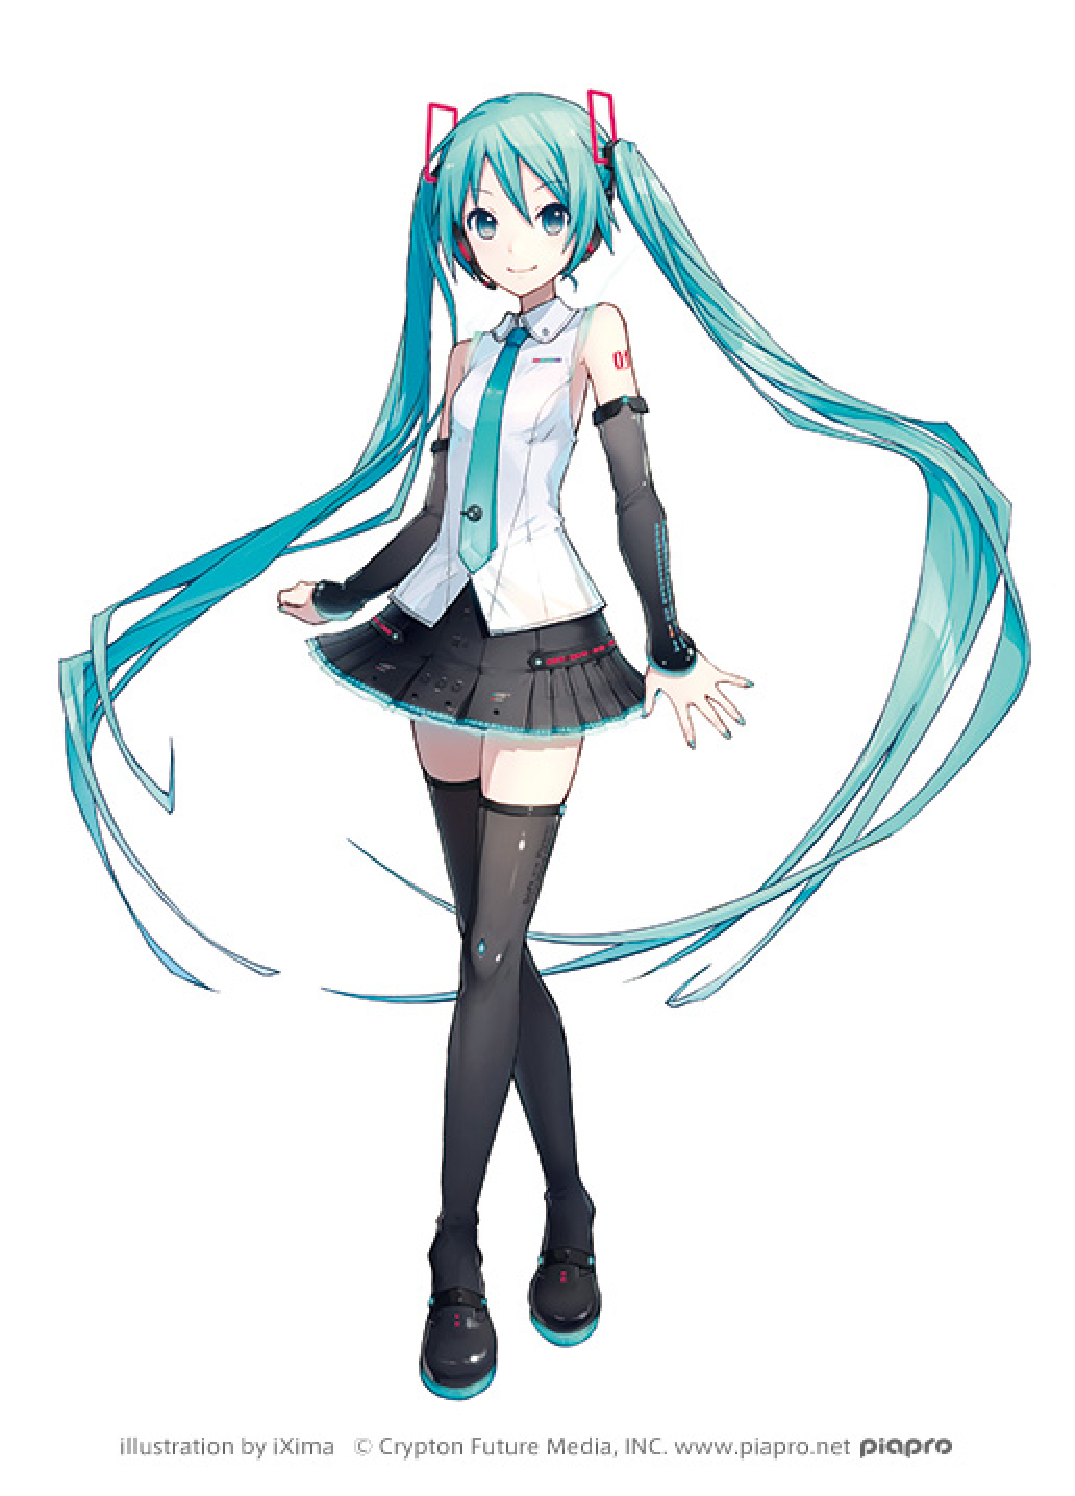
\includegraphics[scale=0.2]{./hatsune.eps}
      \caption{VOCALODの代表格「初音ミク」の最新版V4Xイメージ}
      \label{fig:vocaloid}
    \end{center}
  \end{figure}
\item コンピュータと芸術という分野の一番身近な事象だと思うから\\
音楽は芸術の分野の中でも代表的なものの一つである。しかし、音楽をするためには細かい理論や楽器が演奏できなければいけないなどと思い、敷居が高いものだと感じる人が多い。しかし実際に音楽は音声の高低や長さなどを組み合わせれば、細かい理論などを抜いても音楽といえてしまうほど実は敷居が低いものである。\\
そして、視覚的に操作ができるDTMの登場により、その敷居はさらに低いものになっていった。\\
\end{itemize}
以上の理由から私はDTMについてもっと広く知ってもらいたいと思い、今回技術レポートとして
執筆した。\\
\section{DTMの概要}
\subsection{DTMとは}
\label{sec:aboutdtm}
DTM(ディーティーエム)とはDesk Top Musicの略称であり、コンピュータを用いて楽曲制作を行うことである。わかりやすく例えると、自分の持っているパソコンが音楽スタジオに変身したようなものだと考えればよい。このように言うとだいぶ大げさに聞こえるが、実際コンピュータの中にスタジオ同然の環境を構築するのだから、まったく同じことが言えてしまう。\\
\subsection{どのように曲を作るのか}
\label{sec:howmake}
DTMでの楽曲制作は、コンピュータにインストールしたDAW(Digital Audio Workstation)\footnote{DAWに関しては\ref{sec:DAW}を参照}を中心に合成音源(サウンドフォント)を利用したり、実際に楽器の音声を録音したりして進めていく。やっていることは本当に現実の音楽スタジオと相違ない。\\
\subsection{使用機材}
DTMに必要な機材はいくつかあるが、さわりだけもやってみたい場合にはノートパソコン一台あれば充分である。以下に一般的に使用されている機材を列挙した。\\
\subsubsection{パソコン}
パソコンはDTMをやるうえではなくてはならない必須のツールである。DTMを行うには複数の楽器の音源を同時並行でかつ、リアルタイムで再生処理をしなくてはならないのでそれなりのCPU性能が求められる。また、キャッシュも大量に発生するのでメモリも容量が大きいものを搭載している必要がある。さらに、完成した音楽を保存することはもちろん、作業工程でできる多数のバックアップファイルも保存する必要があるので、記憶容量も大きいほうが望ましい。
\begin{figure}[htbp]
  \begin{center}
    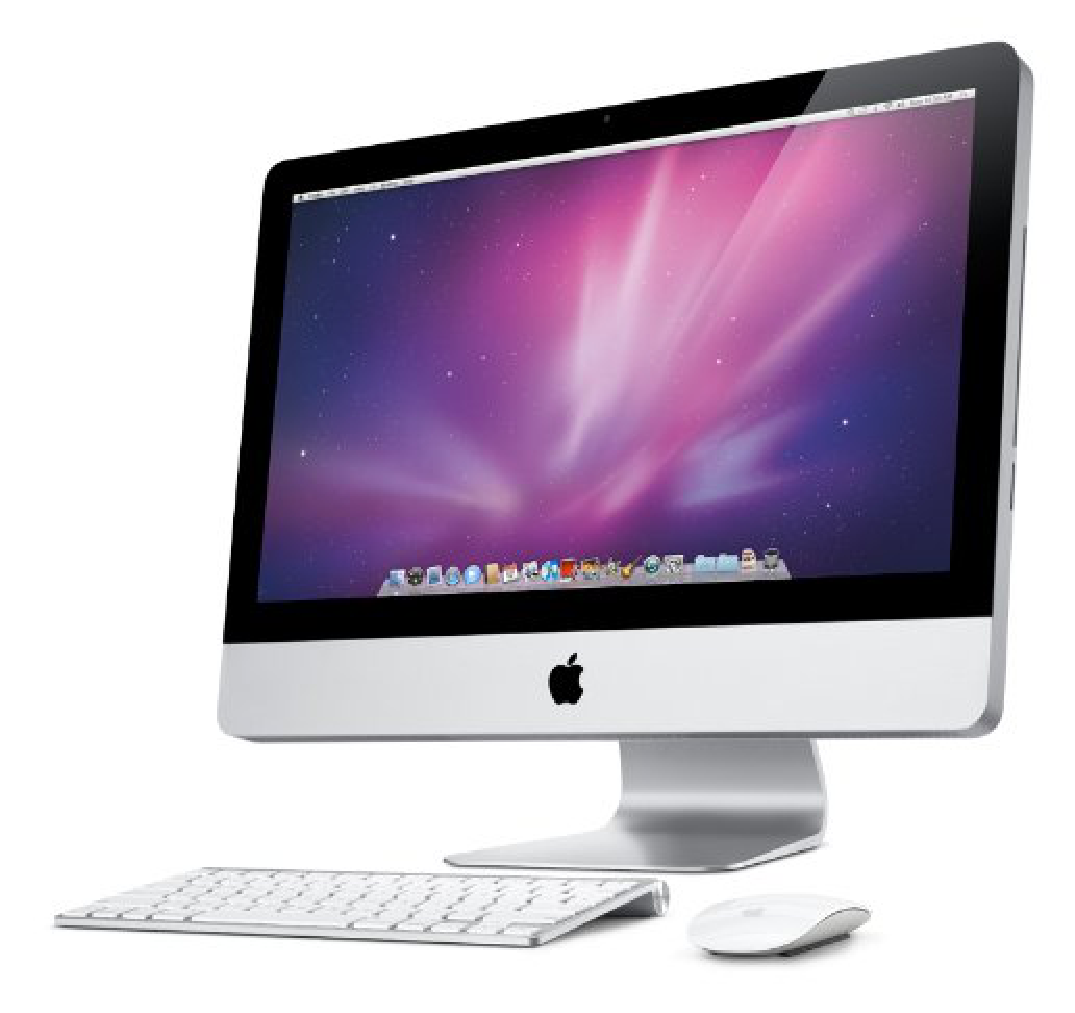
\includegraphics[scale=0.2]{./mac.eps}
    \caption{クリエイター御用達のMac}
    \label{fig:mac}
  \end{center}
\end{figure}
\\
\subsubsection{DAW}
\label{sec:DAW}
DAW(Digital Audio Workstation)とは録音した音源やサウンドフォントの使用、エフェクトをかけるなどDTMをする上ではなくてはならないソフトウェアである。\\
\ref{sec:howmake}で述べたようにDTMはDAWを中心として作業が進められるのでなくてはならないソフトウェアである。\\
近年ではソフトウェアの価格を抑えた初心者向けのものが発売されており、だれでも始めることができるほか、機能は絞られているがプロも使用するレベルのものが無料で始められるものまで登場している。私もDTMに出会った当初はこちらのStudio Oneを使っていた。(図\ref{fig:freedaw})\\
\begin{figure}[htbp]
  \begin{center}
    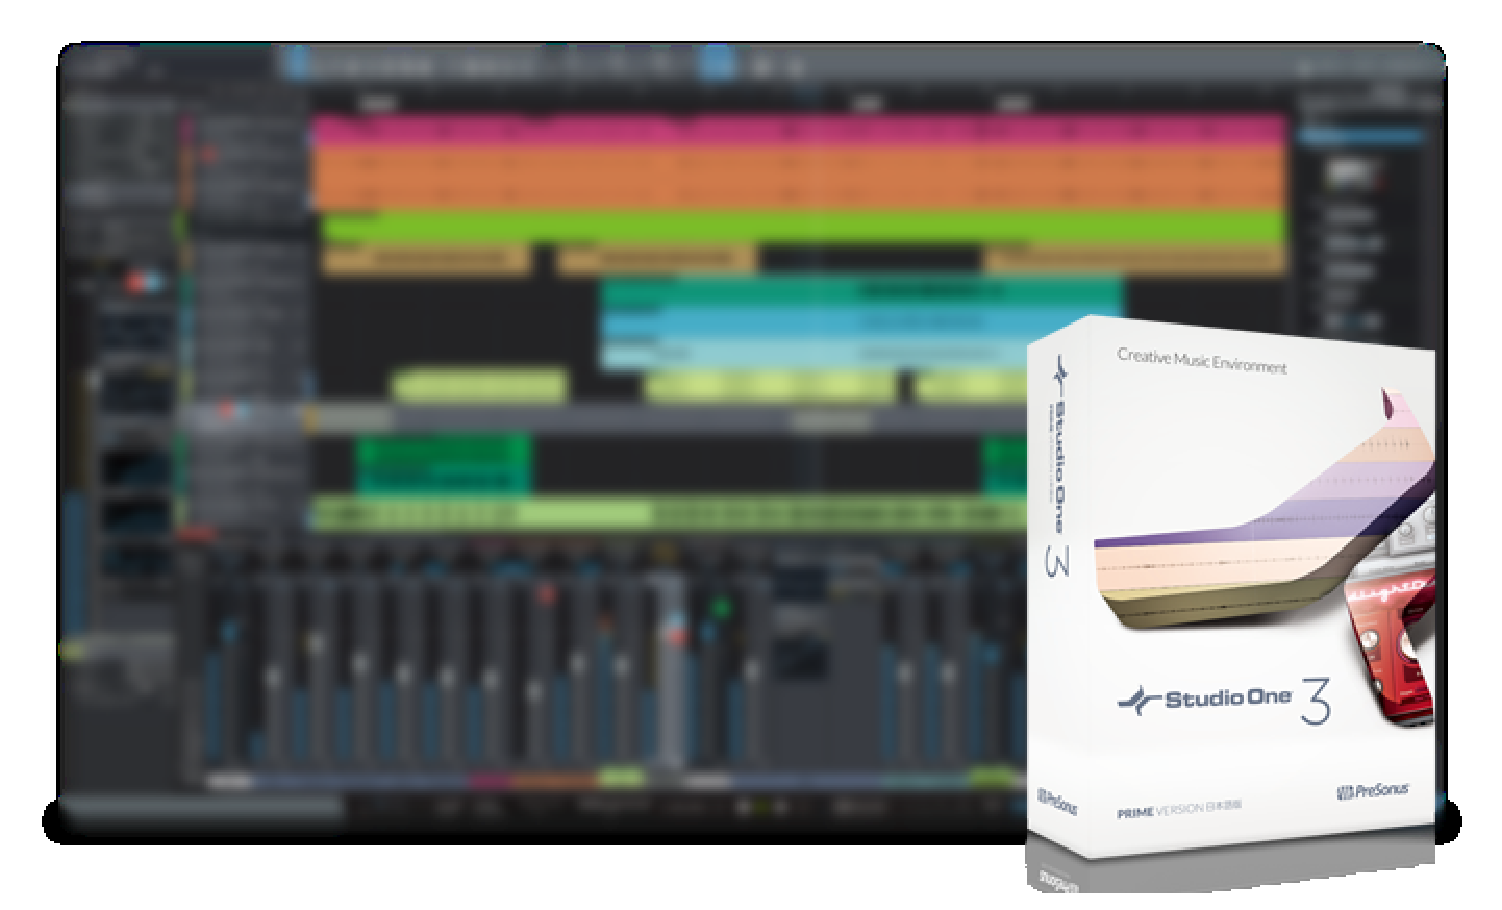
\includegraphics[scale=0.2]{./prime_studio_one.eps}
    \caption{無料だが非常に高品質なStudio One3 Prime}
    \label{fig:freedaw}
  \end{center}
\end{figure}
\subsubsection{MIDIキーボード}
MIDIキーボードは図\ref{fig:key}の様にピアノの形になっており、実際に弾きながら録音や音の確認ができる。このデバイスは無くても制作には全く支障はないので必要に応じてそろえると良い。
\begin{figure}[htbp]
  \begin{center}
    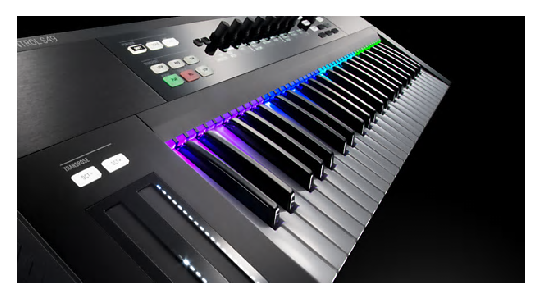
\includegraphics[scale=0.55]{./key.eps}
    \caption{最近の製品は光ったりとデザイン性も高い}
    \label{fig:key}
  \end{center}
\end{figure}\\
\subsubsection{オーディオインターフェース}
オーディオインターフェース(図\ref{fig:audioI})は外部からマイクを繋げたり、編集中の音を聴いたりするために使用する。パソコン(特にノートパソコン)はオーディオ端子が一つ程度しかついておらず、またその性能も非常に低い。(内部のノイズが混じるなど)そのため、音声をUSBを経由して内部のノイズの影響を受けない外部で受け渡しを行うのがこのデバイスである。\\
\begin{figure}[htbp]
  \begin{center}
    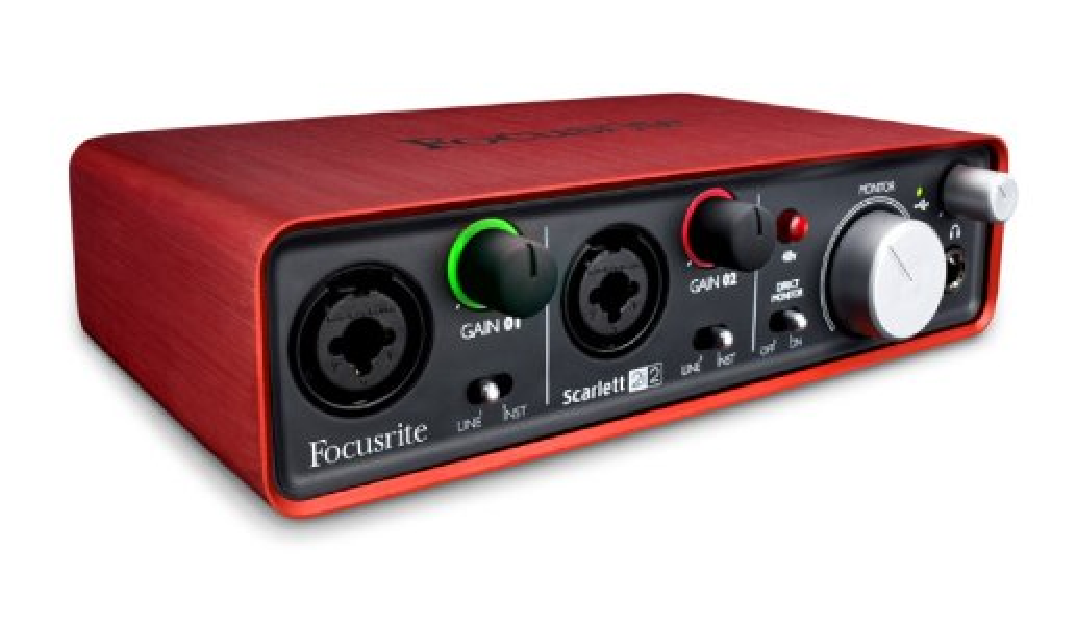
\includegraphics[scale=0.3]{./audioI.eps}
    \caption{手のひらサイズで安価なものもある}
    \label{fig:audioI}
  \end{center}
\end{figure}
\subsubsection{スピーカー・ヘッドフォン}
スピーカーとヘッドフォンは編集中の音を聞くのには欠かせないものである。特にヘッドフォンは夜間の夜業などで音量が出せない環境でも、満足した音量で聞くために必須である。\\
\begin{figure}[htbp]
  \begin{center}
    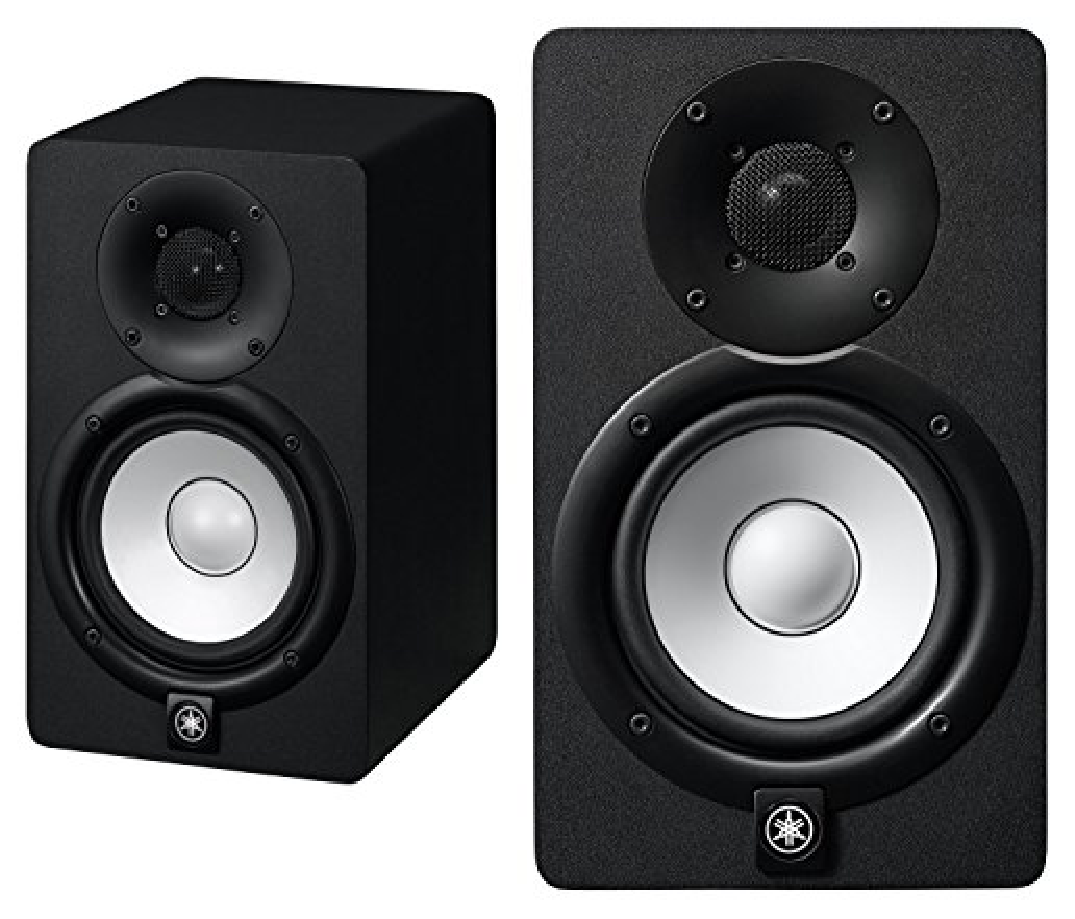
\includegraphics[scale=0.2]{./speaker.eps}
    \label{fig:speaker}
  \end{center}
\end{figure}

\section{DTMの歴史}
\subsection{DTMの確立}
そもそも、この「DTM」という言葉はどこから生まれたのか。調べると、1988年に発売されたRoland社の「ミュージくん」(図\ref{fig:musikun})というDAWの原形のようなものが初めだといわれてる。\cite{melorepi}
また、当時はコンピュータの性能(特にCPU)が今ほど良くはなかったので、リアルタイムでサウンドフォントを生成することが難しかったため、次項で説明する「MIDI」と「シーケンサー」という補助装置を使って作業を拡張していた。\\
\begin{figure}[htbp]
  \begin{center}
    \includegraphics[scale=0.75]{./musikun.eps}
    \caption{ミュージくんの実際のパッケージ}
    \label{fig:musikun}
  \end{center}
\end{figure}

\subsection{MIDIとは}
MIDIについては\cite{dtmstation}によると
\begin{quotation}
  MIDIは、Musical Instruments Digital Interfaceの略で、1981年に策定された電子楽器同士を接続するための世界共通規格です。そう30年以上も前に誕生した規格で、当時、ヤマハ、ローランド、カワイ、コルグの日本メーカー4社と、当時のシーケンシャル・サーキット、オーバーハイムの米メーカー2社の計6社の合意によってまとまったものなのです。
\end{quotation}
とある。30年前以上前というとちょうどミュージくんが発売されたころと重なる。よってMIDIはDTMの初期からある最古参の規格である。\\
MIDI規格で接続された電子楽器間やコンピュータでは何が転送されているのかというと、音階情報を転送し合っている。それらを機器間で共有し合うことにより、楽曲を制作していった。\\
\subsubsection{MIDIはオワコン?}
MIDIはDTM確立初期からある由緒正しい規格であり、非常に画期的である。しかし、コンピュータの性能向上は著しく、特にCPUの性能は2年に10倍の速度で性能が向上しているといわれている。よって30年前に補助要員として使用されていたMIDIも現代では必要がなくなっているのが実情である。\\
本来、楽器の音源(サウンドフォント)は外付けHDDのようにハードウェアとして拡張していくのだが、現代ではそのHDDの容量拡大などに伴い、ソフト音源としてコンピュータに直に内蔵してしまうのが主流となり、わざわざ外部からMIDIを使って同期させる必要がなくなってしまっている。また、USBという万国共通の万能でメジャーな接続規格の普及に伴いMIDIを使用する場合もUSBにとってかわられている。\\
今ではMIDIはもう古いという認識を持つ人も多く、最近始めた初心者などではそもそもMIDI自体を知らないということもある。\\
\subsection{シーケンサーとは}
シーケンサーについては\cite{yoridokoro}によると
\begin{quote}
  MIDIシーケンサーはMIDIデータを打ち込み再生する所です・・・\\
  あなたの代理演奏者です。\\
\end{quote}
とある。シーケンサーの中には楽器の音源(サウンドフォント)情報を受け取り、その音で演奏させるプログラムが実装されており、前項のMIDIと接続し、信号を共有させることで任意の楽器の音源で演奏させることが可能になる。\\
ちなみにシーケンサー単体では基本的演奏させることは不可能である。\footnote{ソフト音源というあらかじめ内蔵されている場合はそれを指定することで可能}\\
\subsection{現代のDTM}
現代ではコンピュータの性能もだが、ソフトウェア自体やDTM環境も目覚ましい発展を遂げている。\\
かつては部屋いっぱいに機材を並べ、MIDIで繋いで制作するのが一般的であったが、現代ではDAW一つにすべての機能が集約されているので、最小環境ともなればノートパソコンだけあれば立派なDTM環境が整ってしまう時代になった。\\
また、音源の加工も容易になりUIを使ってユーザー自身で一から音源を作ることもできるようになった。複雑な処理もDAWが一括して担ってくれるので、遥かに制作の自由度が高くなっている。\\
\begin{figure}[htbp]
  \begin{center}
    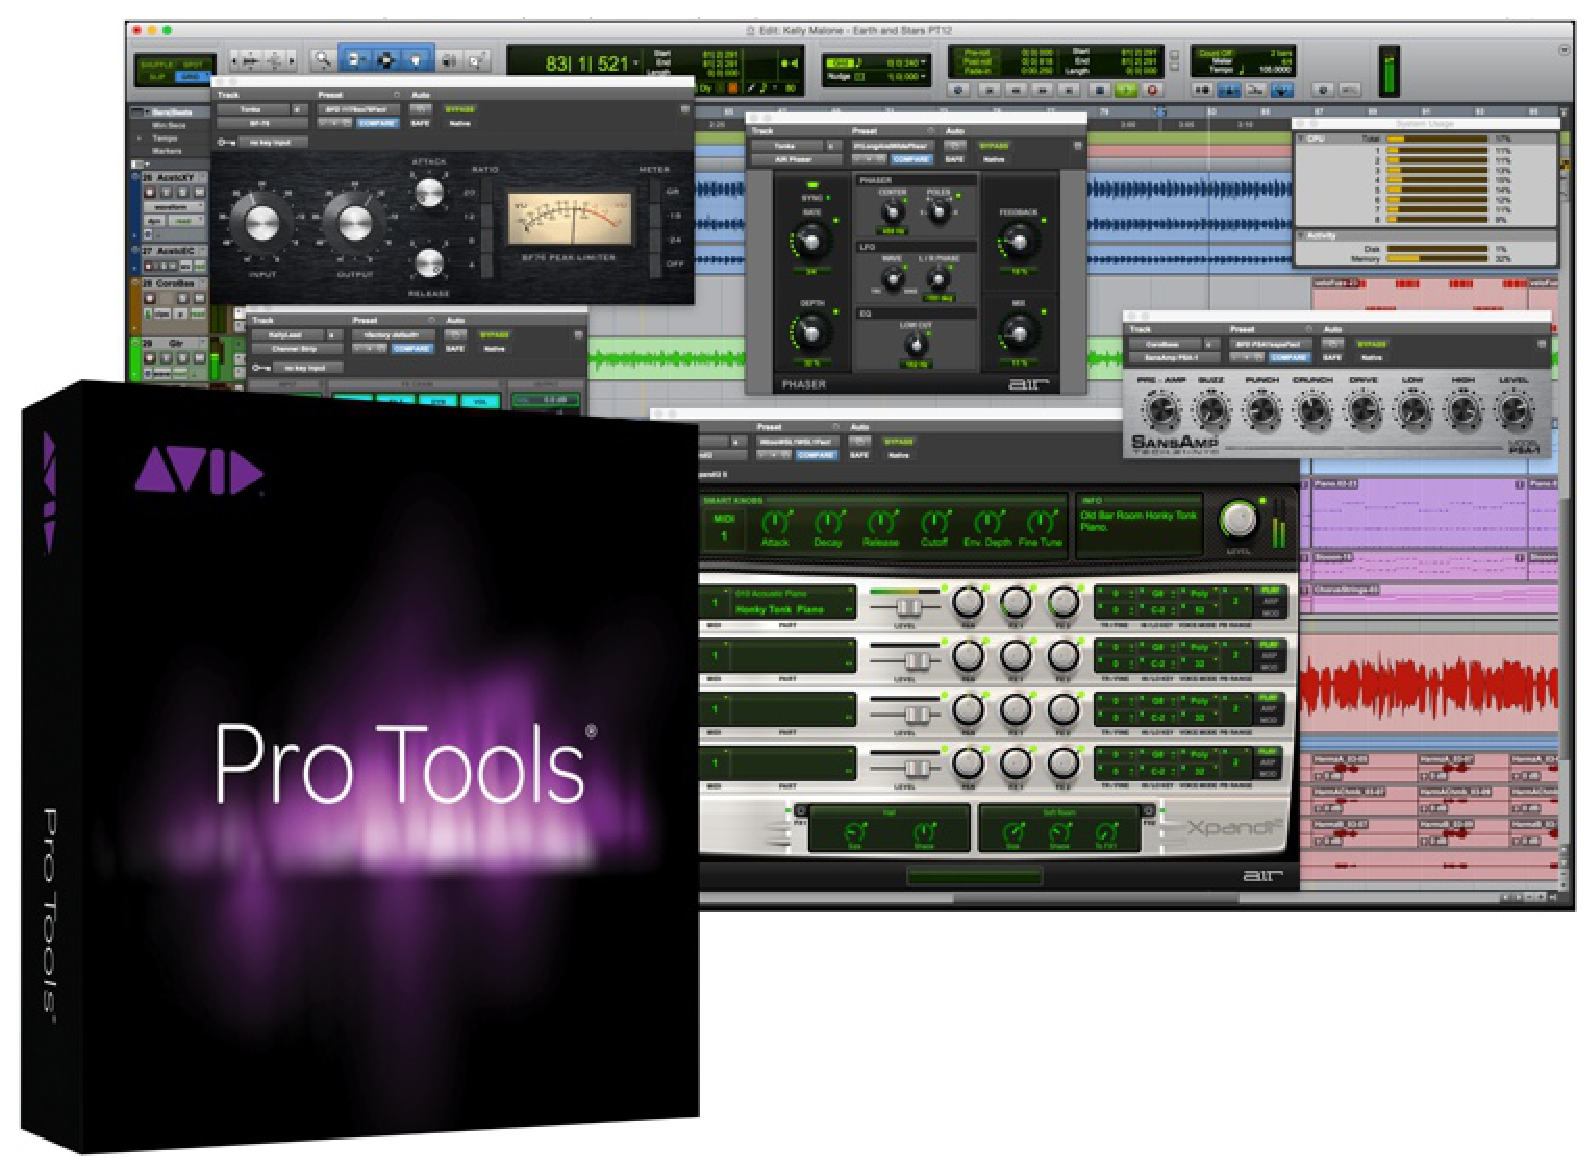
\includegraphics[scale=0.2]{./protools.eps}
    \caption{世界シェアNo1のDAW -Pro Toolsシリーズ-}
    \label{fig:protools}
  \end{center}
\end{figure}
\section{最後に}
私はコンピュータと芸術という分野において、DTMはとても革新的な技術であると考えている。また、その進歩もコンピュータが進化する速度に合わせて進化しており、常に最先端の制作環境で芸術が生まれているといっても過言ではない。DTMは顕著に今後の研究の成果によっては、今回紹介したDTMもさらなる技術的躍進があるに違いない。\\
私は音楽と出会ってDTMを知り、DTMでコンピュータと芸術について理解と興味を広げてきた。この大学でもDTMに特化しているわけではないが、コンピュータと芸術、その中でも「音」の分野に特化した研究をしている場所がある。それくらいコンピュータと芸術は研究対象として価値がある分野である。\\

\bibliography{academic-report}
\end{document} 
